\documentclass[journal, compsoc]{IEEEtran}

\usepackage{graphicx}
\usepackage{algorithm}
\usepackage{algpseudocode}
\usepackage{amsmath}
\usepackage{amsfonts}
\usepackage{hyperref}
\usepackage{mathtools}
\usepackage[euler-digits,euler-hat-accent]{eulervm}

\bibliographystyle{IEEEtran}

\DeclareMathOperator*{\argmin}{arg\,min}
\newcommand\Mycomb[2][^n]{\prescript{#1\mkern-0.5mu}{}C_{#2}}

\title{Artificial Intelligence Report on Solutions to Laboratory Problems}

\author{Siddhartha~Tiwari, Siddharth~Mani~Tiwari, Saurabh~Kumar, Pushkar~Tiwari}

%\author{
%\IEEEauthorblockN{Siddhartha Tiwari}\IEEEauthorblockA{201851127}
%\and
%\IEEEauthorblockN{Siddharth Mani Tiwari}\IEEEauthorblockA{201851126}
%\and
%\IEEEauthorblockN{Saurabh Kumar}\IEEEauthorblockA{201851113}
%\and
%\IEEEauthorblockN{Pushkar Tiwari}\IEEEauthorblockA{201851095}
%}

\begin{document}
\IEEEtitleabstractindextext{%
\begin{abstract}
This report is the part two of discussions on laboratory problems assigned to us by Dr. Pratik Shah. The problems discussed are from various fields including Hidden Markov Models, Markov Random Fields, Hopfield Networks, Unsupervised Learning, N-Arm Bandit e.t.c. For each problem, the most efficient solution is arrived upon gradually, using different techniques taught in the class.
\end{abstract}
}
\maketitle

\section{Hidden Markov Models and Expectation Maximization}
\subsection{Expectation Maximization for finding the Bias of bent coins}
\subsubsection{Introduction}
This problem is to find out the unknown biases of bent coins using the results of random experiments done on the coins.
We can "guess" the biases of coins smartly using Expectation Maximization, which uses the maximum likelihood along with some guesses
to find a more "educated" guess. It uses recursion to improve the guesses. The algorithm is explained in the next subsection for $10$ biased coins.
\subsubsection{The Expectation Maximization algorithm}
In this algorithm we have to start with an intial guess of the biases of the coins. Let the biases be $\hat{p}_{1}$, $\hat{p}_{2} \ldots$, $\hat{p}_{10}$ for the $10$
bent coins given in the problem. These biases represent the probability to obtain $1$ (heads) when the coins are tossed. In each iteration the algorithm
have two steps, the E-step and the M-step.

In the E-step, we calculate that what the probability is, that a certain coin was picked, given the obeservation sequence. This probabilities can be
calculated easily using Bayes theorem. Assume that $O$ represents the observation sequence and the coins are numbered from $1$ to $10$, then the
probability that coin $1$ was used to get $O$ is given by:
\begin{equation}
\label{eqn:bayes}
    P(C = 1 | O) = \frac{P(O | C = 1) \cdot P(C = 1)}{P(O)}
\end{equation}
In the equation \ref{eqn:bayes}, we have used the Bayes theorem to obtain the probability in terms of likelihood, prior and evidence. Now,
since all the coins are equally likely to choose, ${P(C = 1) = \frac{1}{10}}$. Also, P(O) can be rewritten by marginalizing on all the coins:
\begin{equation}
\label{eqn:marginalization}
\begin{aligned}
P(O) &= \sum_{C = 1}^{10} P(C, O) = \sum_{C = 1}^{10} P(O | C) \cdot P(C)\\
&= \frac{1}{10} \sum_{C = 1}^{10} P(O | C)
\end{aligned}
\end{equation}
because, ${P(C) = \frac{1}{10} \hspace{1mm} \forall \hspace{1mm} C \in \{1, 2, 3 \ldots 10\}}$.

So, using the result obtained in the equation \ref{eqn:marginalization}, equation \ref{eqn:bayes} can be rewritten as:
\begin{equation}
\label{eqn:final}
\begin{aligned}
P(C = 1 | O) &= \frac{P(O | C = 1) \cdot \frac{1}{10}}{\frac{1}{10}\sum_{C = 1}^{10} P(O | C)}\\
&= \frac{P(O | C = 1)}{\sum_{C = 1}^{10} P(O | C)}
\end{aligned}
\end{equation}

Now, assume that $n$ and $m$ are two parameters that represent number of heads and number of tails respectively, in $O$. Since, the trials are mutually
independent, the probability $P(C = 1 | O)$ is given by:
\begin{equation}
\label{eqn:finale}
\begin{aligned}
P(C = 1 | O) &= \frac{P(O | C = 1)}{\sum_{C = 1}^{10} P(O | C)}\\
&= \frac{\hat{p}_{1}^{n}\cdot (1 - \hat{p}_{1})^{m}}{\sum_{i = 1}^{10} \hat{p}_{i}^{n}\cdot (1 - \hat{p}_{i})^{m}}
\end{aligned}
\end{equation}

All the other probabilities can be calculated similarly. Now, expected number of heads for the coin $x$ in $O$ will be:
\begin{equation}
\label{eqn:heads}
\begin{aligned}
\mathbb{E}[N_{H}] &= n \cdot P(C = x | O) \hspace{2mm}\\
&= \frac{n\cdot \hat{p}_{x}^{n}\cdot (1 - \hat{p}_{x})^{m}}{\sum_{i = 1}^{10} \hat{p}_{i}^{n}\cdot (1 - \hat{p}_{i})^{m}}
\end{aligned}
\end{equation}

We can also obtain the expected number of tails in the same fashion.

\subsubsection{Conclusion}
So, in the E-step we find out the expected number of heads and tails obtained by using the parameters of that particular iteration.

In the M-step we use the expected number of heads and tails obtained in the E-step to get a new estimation of the biases of all the coins.

In Expectation Maximization these two steps are repeated until the value of parameters converge to some certain value. The biases thus obtained
are the best guesses Expectation Maximization can obtain.

We have implemented this expectation maximization in Python(Jupyter Notebook). Also, we found out after some exploration that if
we keep the biases of two different coins the same at the start the biases obtained after the expectation maximization are also
same for the respective coins.
Hence, assuming that every coin has a different bias (initializing the coins with different biases),
the biases obtained are given in the table \ref{table:biases}.
\begin{table}[!h]
\renewcommand{\arraystretch}{0.4}
\caption{Biases of the coins}
\label{table:biases}
\centering
\begin{tabular}{|c|c|c|}
\hline
{\bfseries Coin} & {\bfseries Initial Biases} & {\bfseries Final Biases}\\
\hline\hline
1 & 0.05 & 0.010000\\
\hline
2 & 0.15 & 0.092424\\
\hline
3 & 0.25 & 0.176789\\
\hline
4 & 0.35 & 0.287559\\
\hline
5 & 0.45 & 0.391205\\
\hline
6 & 0.55 & 0.477410\\
\hline
7 & 0.65 & 0.569790\\
\hline
8 & 0.75 & 0.688256\\
\hline
9 & 0.85 & 0.784089\\
\hline
10 & 0.95 & 0.897061\\
\hline
\end{tabular}
\end{table}

\subsection{Expectation Maximization and k-means clustering}
\subsubsection{Introduction}
In $k$-means clustering, we have to divide a set of points in $k$ different groups or sets such that the sum of
squared distances between every pair in each set is minimized. This can be expressed mathematically as:
\[
    \argmin_G \sum_{i = 1}^{k}\sum_{x,y\in G_{i}} \|x - y\|^{2}
\]

This is also equivalent to maximizing the sum of squared distances of points belonging to different groups. But we can use Gaussian Mixture Models (EM clustering) to
do a distribution-based clustering as we show in the next subsection.

\subsubsection{EM clustering}
In EM clustering we take the fact into account, that the set of points given are from different Gaussian Distributions.
Thus, each Gaussian Distribution represents a group or cluster of points\cite{aibook}. And as soon as we know the distribution, we can
apply the Expectation Maximization in a much similar way as we did in the coin-bias finding problem (there we assumed that the
distribution for each coin is a bernaulli distribution). In this particular problem we have to divide the set of points with
real values (although, it could be multiple real values for each data point, and in that case we have to use multivariate
Gaussians to model it) in two groups. Let the two groups are represented with two $1-D$ Gaussians $G_{1}$ and $G_{2}$, having
weights $W_1$ and $W_2$ and given by:
\[
    G_{1}(x | \mu_{1}, \sigma{1}) = \frac{1}{2\pi\sigma_{1}^{2}}\exp^{-\frac{(x - \mu_{1})^{2}}{2\sigma_{1}^{2}}}
\]
\[
    G_{2}(x | \mu_{2}, \sigma{2}) = \frac{1}{2\pi\sigma_{2}^{2}}\exp^{-\frac{(x - \mu_{2})^{2}}{2\sigma_{2}^{2}}}
\]

In the coin-bias finding problem, the parameters were just the probability of getting heads, but in this
instance of Expectation Maximization the parameters are ${\hat{\theta}_{1} = (\mu_{1}, \sigma_{1}, W_1)}$ and
$\hat{\theta}_{2} = (\mu_{2}, \sigma_{2}, W_2)$.\\

In the E-step we find out the probability of each point to be in one of the clusters and then that value will act as the expected assignment
of the point to that cluster. The equation \ref{eqn:gmm} shows how to calculate the probability of point $d$ being in first cluster.
\begin{equation}
\label{eqn:gmm}
P(C = 1 | d) = \frac{P(d | C = 1)\cdot P(C = 1)}{P(d | C = 1)\cdot P(C = 1) + P(d | C = 2)\cdot P(C = 2)}
\end{equation}

Also using the fact that $P(C = 1) = W_{1}$ and $P(C = 2) = W_{2}$ and the probability of each Gaussian the equation \ref{eqn:gmm} can be
rewritten as:
\begin{equation}
\label{eqn:gmmfinal}
P(C = 1 | d) = \frac{W_{1} \cdot G_{1}(d | \mu_{1}, \sigma{1})}{W_1\cdot G_{1}(d | \mu_{1}, \sigma{1}) + W_2\cdot G_{2}(d | \mu_{2}, \sigma{2})}
\end{equation}

Similarly, the probability of point $d$ lying in the second cluster can also be calculated.\\

In the M-step, we use the probabilities calculated above to find out the new values of mean, variance, and weights.

\subsubsection{Conclusion}
EM clustering assumes that the data points follow the Gaussian Distribution. Another way to find out the clustering is the famous K-means algorithm.
In K-means, similar to EM clustering, we initally assume the means and then improve it in each iteration by clustering points according to those means.
This is almost same as what we are doing in EM clustering.

The code of our EM clustering can be found at our GitHub codes repository. The result of the clustering of the points using our EM implementation
is shown in the figure \ref{fig:cluster}.
\begin{figure}[!h]
\centering

\includegraphics[width=2.5in]{images/points.pdf}
\caption{Points to cluster}
\label{fig:cluster}
\end{figure}
\begin{figure}[!h]
\centering
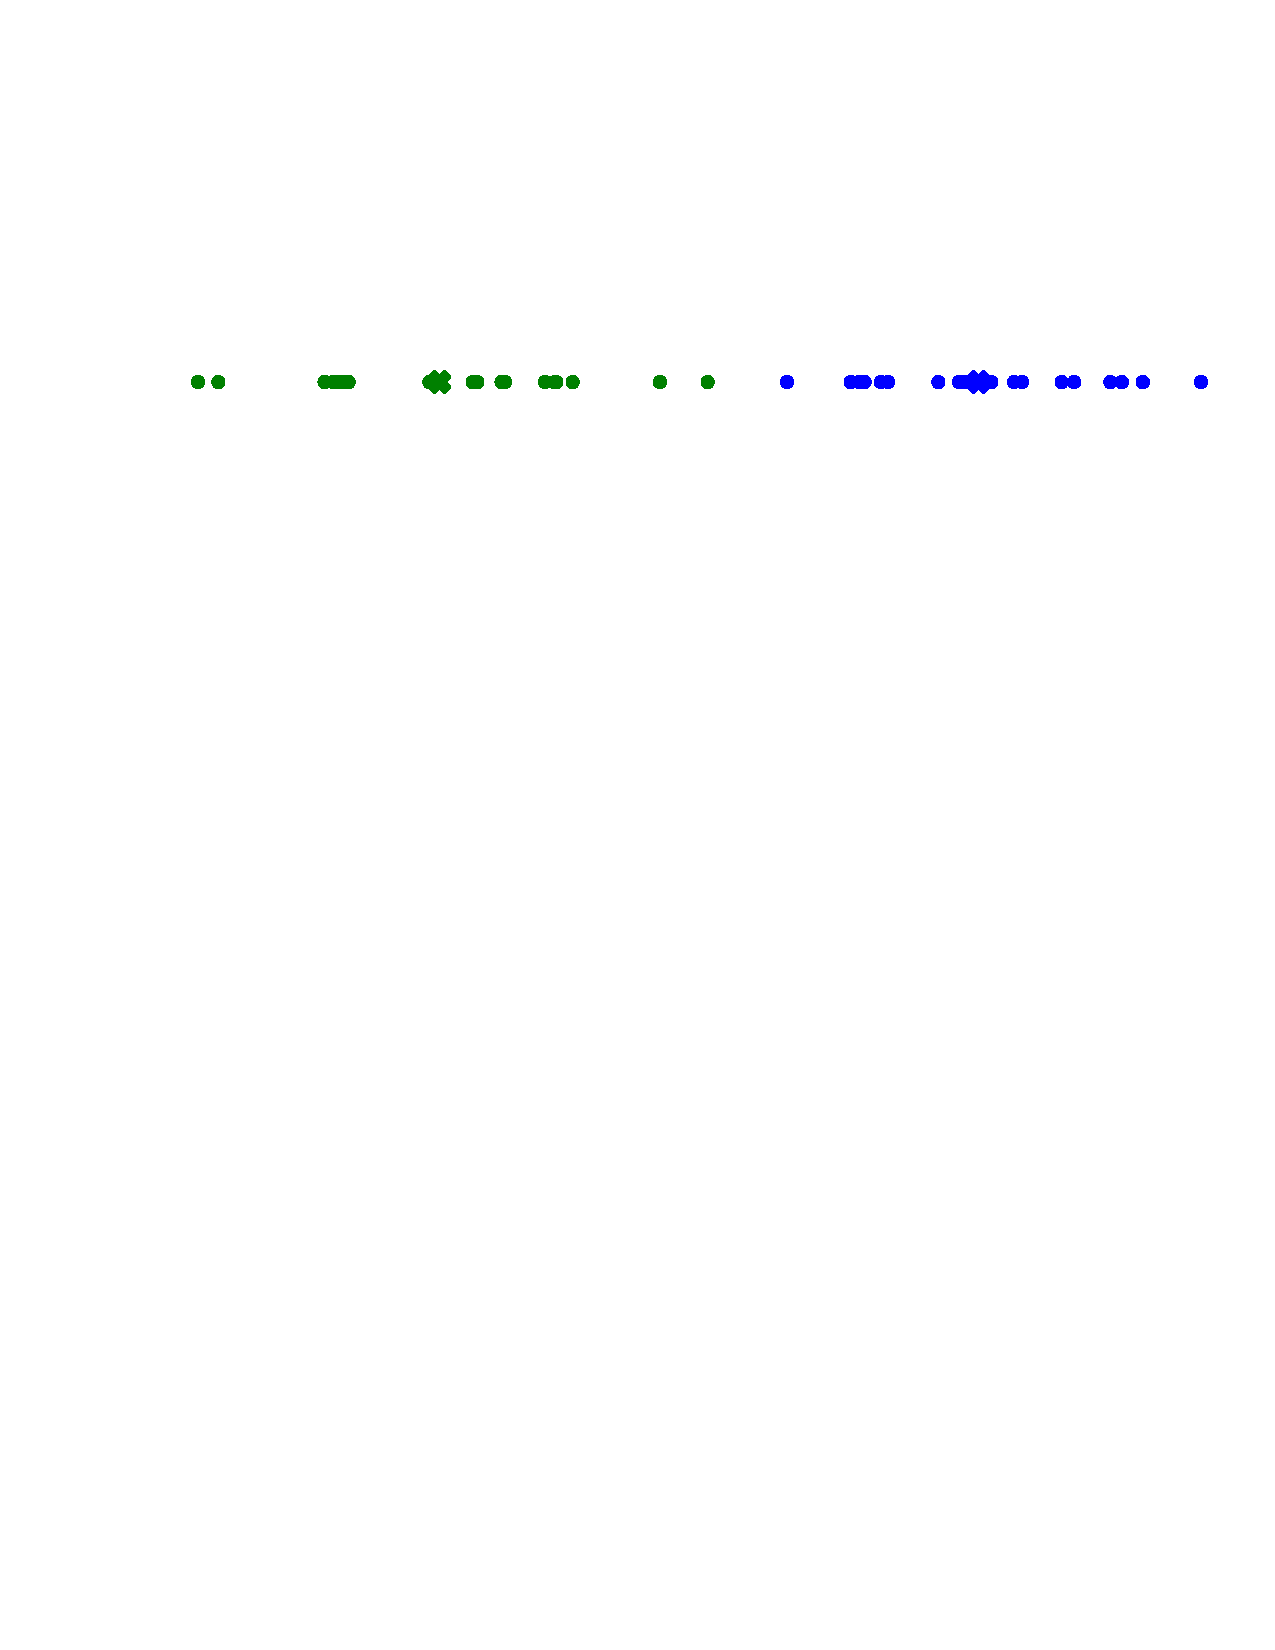
\includegraphics[width=2.5in]{images/clustered_points.pdf}
\caption{Points grouped in two clusters (green and blue). The points labelled with X represent the means of the corresponding distributions}
\label{fig:cluster}
\end{figure}

One interesting thing we found out while implementing the algorithm is that not every start state gives us this clustering. Many start states are a failure.
And I think it must be right too, because EM only finds the local optimum and not the global optimum. If our initial guess is bad then it probably will not
give the optimal value of the means. The means, variance and weights of the two Gaussians are given in the table \ref{table:parameters}.

\begin{table}[!h]
\renewcommand{\arraystretch}{0.4}
\caption{Parameters of the Gaussians}
\label{table:parameters}
\centering
\begin{tabular}{|c|c|c|c|}
\hline
{\bfseries S.No.} & {\bfseries Mean} & {\bfseries Variance} & {\bfseries Weight}\\
\hline \hline
1 & 0.7062 & 0.7155 & 0.5010\\
\hline
2 & 4.0404 & 0.4763 & 0.4989\\
\hline
\end{tabular}
\end{table}
\nocite{Do2008}
\nocite{HMM_Stamp}
\bibliography{references}
\end{document}
